\documentclass[final]{IEEEtran}
\usepackage{cite}
\usepackage{amsmath,amssymb,amsfonts}
\usepackage{algorithmic}
\usepackage{graphicx}
\usepackage{textcomp}
\usepackage{xcolor}
\usepackage{datetime}
\usepackage{seqsplit}

\graphicspath{{./images/}}
\def\BibTeX{{\rm B\kern-.05em{\sc i\kern-.025em b}\kern-.08em
    T\kern-.1667em\lower.7ex\hbox{E}\kern-.125emX}}
\begin{document}

\title{ Scam Booter\\\vspace*{10pt} \LARGE CPEN442 \\\vspace*{10pt} \large October 11}
\author{\textbf{Zoy Huang (20026150), Ryan Koon (11062149), and Wendy Zhou (41378150)}\\
Department of Electrical and Computer Engineering\\
University of British Columbia\\
Vancouver, Canada

%\\\vspace*{10pt}
%emailA.com, emailB.com, emailC.com
}
\maketitle

% The abstract should summarize the problem addressed, methodology, results, conclusions, and contributions.
\begin{abstract}
\end{abstract}

\section{Introduction} % 10%
%================================================================================================================
%The section should provide the following
%
%1. Explain clearly the problem addressed by your project.
%2. Explain why this is an important problem.
%3. Summarize the designed system
%4. Summarize related work.
%5. Summarize the methodology that you have followed for evaluating your design.
%6. *Summarize evaluation results you obtained .
%7. *Summarize the conclusions your drew from the results.
%8. List contributions of your project.
%
% *Only for the final Report
%================================================================================================================

\subsection{What is the problem that we addressed?}
%===============================
We addressed the issue of social engineering from technical support scams, which has caused an increasing trend of reported financial losses \cite{b1}. We proposed a solution that protects users with little knowledge about Windows' administrative tools. The asset at risk is the victim's bank account. The vulnerability is the victims lack of knowledge about Administrative tools on Windows. The threats are people pretending to be legitimate technicians and deceiving users about the state of their computer.

\subsection{Why is this problem important?}
%===============================
According to Microsoft, there were 153,000 technical support scam reports worldwide in 2017, a 24\% growth from the previous year \cite[Fig 1]{b3}. In the same year, the Internet Crime Complaint Center (IC3) received approximately 11,000 technical support complaints that totals to a loss of almost \$15 million. That was an “86\% increase in losses from 2016” \cite{b1}.

\begin{figure}[htbp]
\centerline{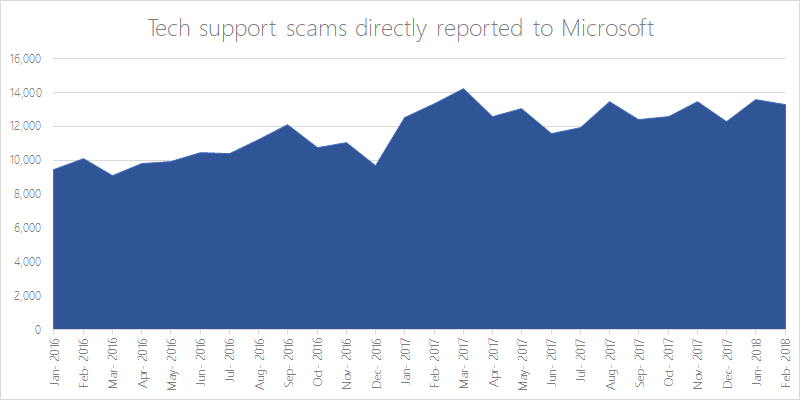
\includegraphics[keepaspectratio=true, scale = 0.32]{image1.png}}
\caption{Number of tech support scams reported to Microsoft}
\label{fig2}
\end{figure}

A study \cite{b2} conducted in 2014 discovered 1,688,412 unique visitors to scam sites and estimated a loss of at least \$9.7 million. With this trend, it appears that technical support scams are not going away even with efforts to stop them \cite[p. 8]{b2}.

\begin{figure}[htbp]
\centerline{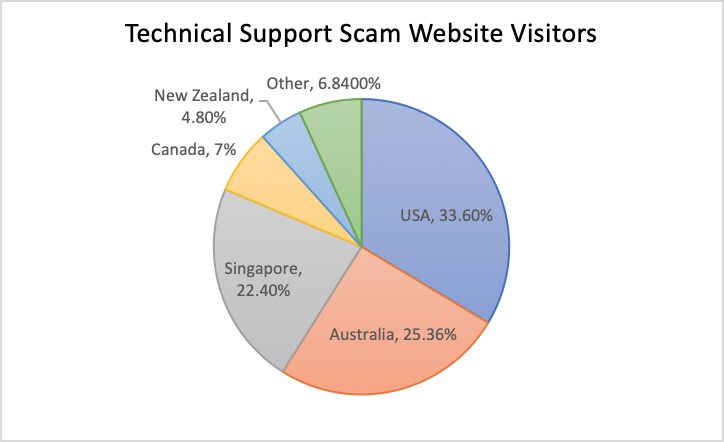
\includegraphics[keepaspectratio=true, scale = 0.30]{image0.png}}
\caption{Tech support scam website visitors by country}
\label{fig1}
\end{figure}

\subsection{Summary of the Designed System}
%===============================
Social engineering attacks thrive on human error based on an inadequate knowledge of the system being used. A novice user does not have the knowledge to recognize fallacies provided by the technical support scammer, nor do they have working knowledge of Windows tools used to manipulate them.

However, notably, scammers follow similar sequences of events and use similar techniques to convince their victims. The most common techniques are shown in \cite[Fig 3]{b2}.
\begin{figure}[htbp]
\centerline{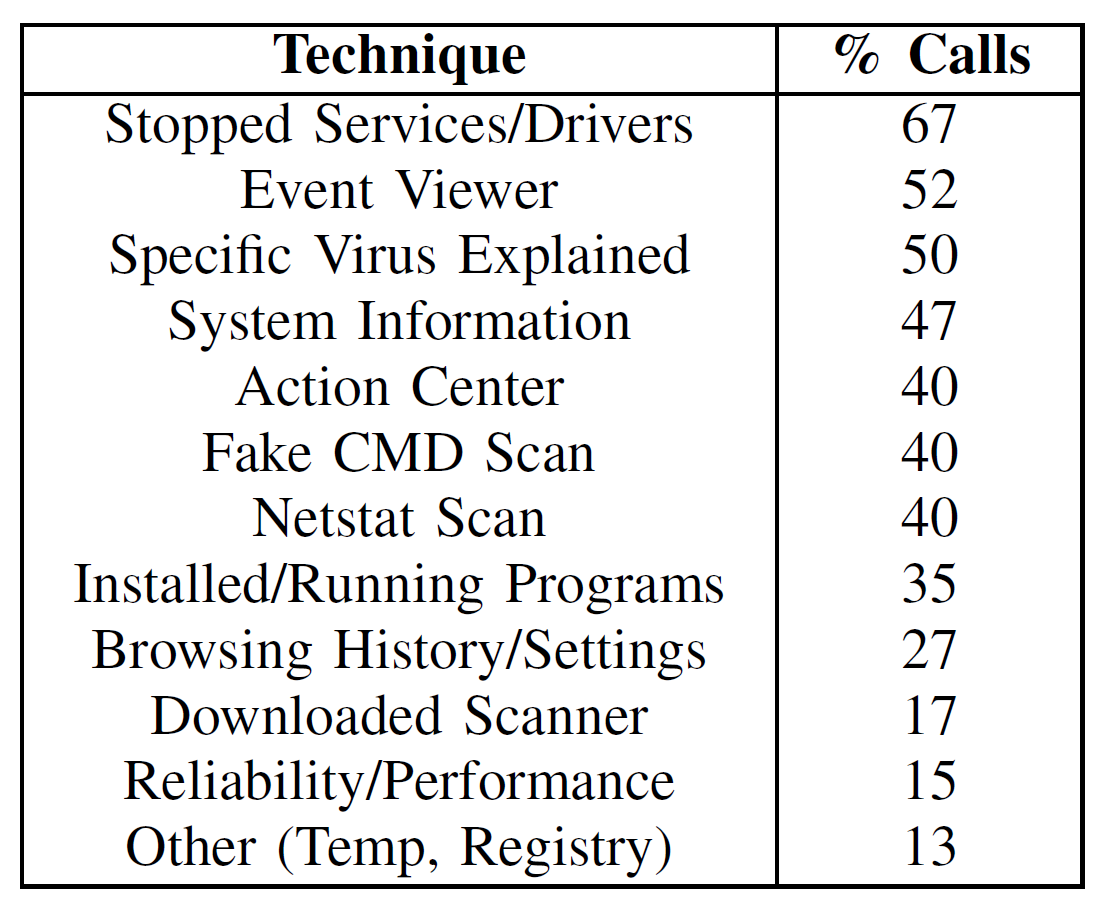
\includegraphics[keepaspectratio=true, scale = 0.20]{image3.png}}
\caption{Techniques used by support scammers in order to convince their victims of a malware infection}
\label{fig3}
\end{figure}

We defined these events and techniques as ``suspicious behavior''. For example, the use of the administrative tool, ``Event Viewer'', qualifies as suspicious behavior. Our solution protects users that lack knowledge about the tools and techniques used in technical support scams by detecting these events on their behalf.

We addressed the problem by using the Windows API to build a Windows application that detects the suspicious behaviors. If a scam is detected, the application forcefully terminates any remote connections and informs the user of the event. We also explored options to prevent the application from being terminated. An option was to create a Windows service that manages the lifecycle of the application. There are other methods to make it even more difficult to shut down the application. However, those methods would likely be flagged by an antivirus solution. To ensure our application is compatible with antivirus programs, we uploaded our application binaries to VirusTotal to be analyzed by 68 antivirus scanners.

\subsection{Summary of Related Works}
%===============================

ROBOVIC, short for Robotic Victim, was a tool created in a study that collected data about technical support scams. It crawled the web to find websites, its visitors, and phone numbers used for these kinds of scams \cite[Fig 2]{b2}. The investigators concluded that “the vast majority of AV users are likely not going to be protected against technical support scams”  \cite[p.7]{b2}. On average, 64\% of 1624 malicious TLDs (Top Level Domains) were only detected by 3.25 AV engines out of 68 engines \cite[p.7]{b2}. Phone applications on Android detected “less than 1\% of the 1,581 scammer-operated phone numbers” \cite[p.8]{b2}. On average it took 44 days for a phone number to be reported as a part of a scam. Even worse, some mobile applications associated scam numbers with positive reviews and legitimate businesses such as Dell and McAfee. Microsoft has been making a wide range of improvements by “enhancing antivirus, email, URL blocking, and browser security solutions”. TeamViewer has been displaying prompts to warn users about technical support scams. In terms of user education, attempts such as public service announcements have been made. However, they were ineffective being on specific sites that were not known by the general population  \cite[p.13]{b2}.


%NOTE: Should probably get some academic sources for this section, and rewrite it. +++++

\subsection{Summary of the Methodology}
%===============================
We constructed a test suite that contains various forms of unique and documented technical support scams. For each scam, we made many similar attacks against a system protected by our solution. We assessed the effectiveness of our solution based on the number of detected attacks in the test suite.

%\subsection{Summary of Evaluation Results}
%===============================
% %Only for the final Report

%\subsection{Summary of our Conclusion}
%===============================
% %Only for the final Report

% Existing solutions include informing the user through online information, blacklisting scammers' numbers and domain names, and antivirus solutions. Blacklisting scammer websites and phone numbers is not an effective method since the scammers can always register new domain names, create new websites, and use other phone numbers. Our solution focused on detecting a potential scam on the user's system and immediately brings them back to safety. It protects users who are experiencing potential phone scams and does not rely on numbers and IP addresses of scammers. The goal of our system was not only prevention but also detection and recovery. This can be considered a layer of defense inside a “fortress”, which helps protect inexperienced users.

\subsection{List of Contributions}
%===============================


\section{Related Work} % 5%
%================================================================================================================
% This section should explain what others, particularly as reported in academic literature, have done designing systems similar to the one designed by your team.
%================================================================================================================





\section{Adversary Model} % 9%
%================================================================================================================
% Describe the adversary model that your design is intended to resist.
%================================================================================================================
Although there are various techiniques that are used by technical support scammers, we developed a generalized model by analyzing the patterns of technical support scams. This model facilitated our understanding of the problem and helped us to design our system.
\subsection{Objectives}
The objective of the adversaries is to convince the victim that their computer is infected by a virus. After gaining the trust of the victim, the adversaries make the victim to pay them for fixing non-existent problems. The adversaries are scammers who want to make profits by deceiving inexperienced Windows users.
\subsection{Initial capabilities}
The adversaries can call users, claiming to be from well-known companies. The adversaries can also set up malicious websites or advertisements that tell the user to call technical support numbers. 
\subsection{Capabilities during the attack}
The adversaries ask a user to download remote access software and gain access to their computer. They can open administrative tools to show system "errors", which are logs of normal operation. They can install malwares on the user's machine, causing the machine crash.

\section{System Design} % 20%
%================================================================================================================
% 1. This section should explain the most interesting parts of your design.
% 2. Provide rationale for the design decisions.
% 3. Explain which principles of designing secure systems have been employed by your design.
%===============================================================================================================

\subsection{Detecting a remote connection}
%===============================
Detecting an active remote desktop connection is not as trivial as checking a flag. For Windows, that is only possible if the application is using the Microsoft Remote Desktop Protocol, which operates on specific ports. However, the remote desktop applications used by technical support scammers typically establish connections on port 80 and 443, the standard ports used by web clients to communicate with a machine. Also, these ports are only used to establish a connection, the resulting port is not the same for each session as it is assigned by the machine serving the desktop. Other non-standard ports are used by remote desktop applications, but they differ between software, they may not be documented, or the ports they use will change depending on network conditions. Such a moving target will result in a high rate of false-positives. Instead of analysing network traffic, our application analyses raw input data using the Windows Desktop API \cite {b4}. Every time a mouse click occurs, regardless of the application in focus, our application will check whether a handler to the device is provided in the raw input header. If so, it is a local device that is attached to the computer. If no handler is provided, it is an input made from an active remote connection to the computer. Using this method, we can distinguish between clicks from a locally connected mouse and clicks from a remote desktop application.

\subsection{Detect the use of administrative tools}
%===============================

\subsection{Analysing keystrokes}
%===============================
To improve the accuracy of detecting a scam in progress, we log keystrokes when the Windows Command Prompt is in focus. Scammers frequently execute certain commands to trick the user into believing that there is malware on their computer. 40\% of scammers employ a “Fake CMD scan” by running a command to list the tree of files, folders, and subfolders at a certain path \cite[p.7]{b2}. Our application will capture keystrokes that occur while the command prompt is outputting information. We will look for common words and phrases typed in such as “Virus detected”. We employ this strategy because users are often tricked into believing that the system produced the output not knowing that user inputs are displayed after a command is done executing. To capture keystrokes we use a global hook open source library that will allow our application to learn about keystrokes regardless of the application in focus \cite {b5}.

\subsection{Terminating remote access applications}
%===============================
A fail-safe strategy to terminate the connection between the user and the scammer is to stop all network traffic. However, this will affect all other applications that require network connectivity which arguably, makes our application appear to be malware. To prevent such degradation to the user experience, we terminate common remote desktop applications used by technical support scammers instead \cite[Fig 4]{b2}. Our application runs with elevated privileges to allow us to terminate remote access applications with elevated privileges and to counter process renaming done via a file rename. We access the file metadata to determine the original name of the application rather than relying solely on the process name.

\begin{figure}[htbp]
\centerline{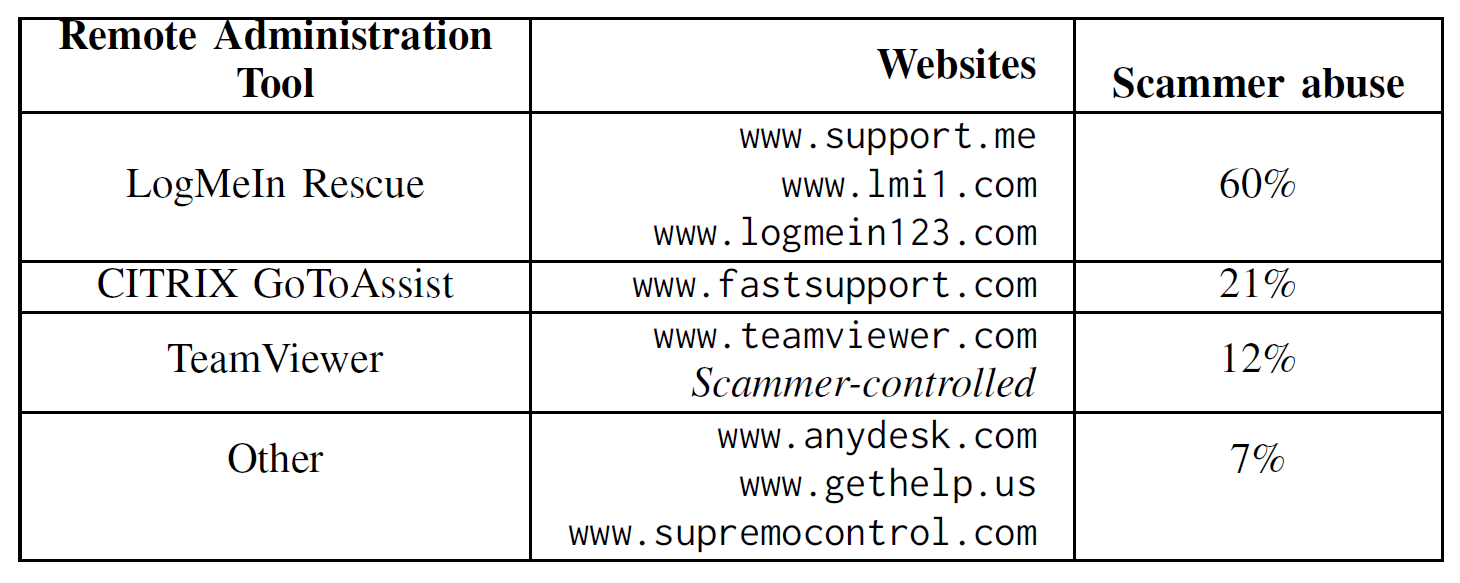
\includegraphics[keepaspectratio=true, scale = 0.22]{RemoteTools.png}}
\caption{Remote access tools used by technical support scammers.}
\label{fig 4}
\end{figure}

\subsection{Self restarting}
%===============================

\section{System Prototype} % 15%
%================================================================================================================
% Explain the details of the prototype of your approach. This is the prototype that is used for evaluating your approach.
%================================================================================================================

\section{Evaluation} % 26%
%================================================================================================================
% This section should provide details of the evaluation, using the following sub-subsections.
%
% 1. (A. Evaluation Methodology) (12%) This subsection should explain how the system was evaluated. Focus on the most important for the reader elements of your evaluation.
% 2. *(B. Results of the evaluation) (7%) This section should describe the results of the evaluation. Remember to keep the description of the evaluation and the description of the results in separate sub-sections.
% 3. *(C. Discussion of the evaluation results) (7%) This section should discuss what the results of the evaluation mean.

%The above enumerated items should be discussed in separate subsections of Methodology section. Their titles are suggested in the parenthesis.
% *Only for the final Report
%================================================================================================================



\subsection{Evaluation Methodology}
%===============================



%\subsection{Discussion} % 10%
%===============================
%%Only for the final Report

%\subsection{Discussion} % 10%
%===============================
%%Only for the final Report







%\section{Discussion} % 10%
%================================================================================================================
% Discuss pros and cons of your design, as well as limitations and advantages of it. This discussion should integrate the related work, the motivation for the design, the adversary model, the ideas of the design, and the results of the evaluation. This section should be about one page. 
%Only for the final Report
%================================================================================================================

%\section{Conclusion} % 5%
%================================================================================================================
% This section should summarize the report in 1-2 paragraphs. Although a conclusion may review the main points of the report, do not replicate the abstract as the conclusion. A conclusion might elaborate on the importance of the work or suggest applications and extensions.
% Only for the final Report
%================================================================================================================


\begin{thebibliography}{00}
\bibitem{b1}  Federal Bureau of Investigation, ``TECH SUPPORT FRAUD'',  https://www.ic3.gov/media/2018/180328, Mar. 28, 2018 [Oct. 6 2018]
\bibitem{b2} N. Miramirkhani, O. Starov, and N. Nikiforakis, “Dial One for Scam: A Large-Scale Analysis of Technical Support Scams,” in Proceedings 2017 Network and Distributed System Security Symposium, 2017
\bibitem{b3} Erik Wahlstrom, ``Teaming up in the war on tech support scams'', https://cloudblogs.microsoft.com/microsoftsecure/2018/04/20/teaming-up-in-the-war-on-tech-support-scams/, April 20, 2018 [Oct. 6 2018]
\bibitem{b4}"C\# Get Mouse handle (GetRawInputDeviceInfo)", Stack Overflow, 2018. [Online]. Available: https://stackoverflow.com/questions/14584280/c-sharp-get-mouse-handle-getrawinputdeviceinfo. [Accessed: 09- Nov- 2018].
\bibitem{b5}"rvknth043/Global-Low-Level-Key-Board-And-Mouse-Hook", GitHub, 2018. [Online]. Available: https://github.com/rvknth043/Global-Low-Level-Key-Board-And-Mouse-Hook. [Accessed: 09- Nov- 2018].
\bibliographystyle{IEEEtran}
\end{thebibliography}

\end{document}
